
\section{Requirements}

\subsection{Who Will Be Served}

The main drive for this completion of this project is Saurabh Chakravarty, our client. By iterating over his feedback, we are treating him as the eventual end user. Eric Williamson is also working with Saurabh as an additional client for the project and a potential end user.  Theoretically there is room for expansion when it comes to future users. If we are successful in “predicting” the stock market, there is potential for our work to be used for monetary gain, but no plan is in place at the current time. 

Automated stock trading is a rapidly developing research area. Our paper will help to further expand this research. Its availability on VTechWorks will allow future researchers to expand upon our work.  As evidenced by our group's use of earlier work done at Virginia Tech through CrowdIQ we can provide an exceptional roadmap to jump start others' forays into utilizing microblogging data as predictive input.  

Formally there are no current plans for extended support. As opposed to other potential projects in this class ours is more conceptual/research based. Hopefully, the ability of others to reference our research will result in its future use.

\subsection{Scenarios Served}

\begin{table}
  \centering
  \begin{tabular}{ | r | l | }
    \hline
    Symbol & Name \\ \hline
    \texttt{\$APPL} & Apple Inc. \\ \hline
    \texttt{\$FB} & Facebook \\ \hline
    \texttt{\$GILD} & Gilead Sciences Inc. \\ \hline
    \texttt{\$KNDI} & Kandi Technologies Group Inc. \\ \hline
    \texttt{\$MNKD} & MannKind Corporation \\ \hline
    \texttt{\$NQ} & NQ Mobile Inc. \\\hline
    \texttt{\$PLUG} & Plug Power Inc. \\\hline
    \texttt{\$QQQ} & PowerShares QQQ Trust, Series 1 (ETF) \\\hline
    \texttt{\$SPY} & SPDR S\&P 500 ETF Trust \\\hline
    \texttt{\$TSLA} & Tesla Inc. \\\hline
    \texttt{\$VRNG} & Vringo Inc. \\\hline
  \end{tabular}
  \caption{Baseline Stocks}\label{tab:stocks}
\end{table}

We are tasked with building an extensible trading simulation software that can be used to define and test any arbitrary trading strategy. This trading software should be able to operate on arbitrary market-related events, such as posts on microblogging websites, stock price changes, and market open and close events.

The simulation software must allow the querying of the most recent stock price for a symbol at a given time. In addition, there must be a comprehensive virtual portfolio implementation that allows strategies to easily execute transactions that buy or sell shares of a stock. The virtual portfolio must take transaction fees into account with every transaction.

We also must implement the opinion aggregation model from \textit{CrowdIQ}. This complex aggregation model takes a judge's historical accuracy and the interdependence of each post into account to accumulate an accurate opinion. This will be used to implement strategies that operate on the perceived market sentiment of a stock.

Our focus is to test and compare the performance of trading strategies for 11 stocks in the year of 2014. These 11 stocks are shown in table~\ref{tab:stocks}. This set of historical data is used to compare our results to a baseline. Focusing our testing to the same set of stocks allows for a more accurate comparisons of performance. Otherwise, the performance of the chosen stocks for a strategy would influence the potential returns.

Our reach goal is to test our strategy on other time intervals in addition to the year of 2014. This will allow us to ensure that our trading method is not created just to specifically fit the data from 2014. This additional testing comes at a much lower cost than going straight to real time testing as it will be quicker and much of the implementation overlaps from the baseline set. 

A prospective future use case of this system is for real-time testing. Real-time access to stock prices and microblogging data often comes at quite a high cost. Therefore, we are not expecting to perform any real-time testing.

\subsection{Data To Be Processed}

\begin{figure}
  \centering
  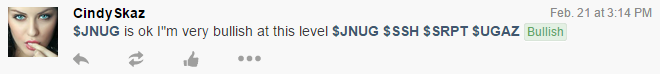
\includegraphics[max width=\textwidth]{stocktwits}
  \caption{Example microblog post from StockTwits}\label{fig:stocktwits}
\end{figure}

As mentioned before, the main dataset consists of microblog posts from the StockTwits website. Each post will contain a stock symbol at the front as a way to determine what stock the user is talking about (see Figure~\ref{fig:stocktwits}). Some posts will also contain a tag referring to the tweet as either bullish or bearish. We will use sentiment analysis to detect the sentiment of untagged posts.

The initial data set will focus on 11 stocks, shown in Table~\ref{tab:stocks}, for the year 2014. However, we hope to expand this time frame to include the year of 2015 as well. This will require us to obtain a set of microblog posts for year of 2015 from StockTwits.

We will use stock price data to verify past predictions by judges. The verification of past predictions will be used to assign a weight to each judge. A judge's weight corresponds to the historical performance of that judge in predicting stock price trends. Additionally, we will use the order in which posts arrive to determine the interdependence of a judge's opinions on other judges. This will be used to prevent judges who are subject to groupthink from affecting the overall market sentiment. All of this judge performance analysis will be implemented from \textit{CrowdIQ}.

By analyzing the portfolio value over time of different strategies, we will determine which strategies perform most optimally. We can further analyze specific large changes in portfolio values to determine why a strategy might have gained or lost money. The prices of the 11 stocks during the change and the microblog posts during the change will be referenced in this analysis.

\subsection{Existing Code Base}

Saurabh and Eric have provided us with some code that will help implement the sentiment analysis. This code is in the Scala general-purpose programming language \cite{scala}. Due to this code already being created we have decided to do the rest of the program in Scala as well and will be storing in on a public GitHub repository.

We will also make use of previous implementations of chosen machine learning algorithms (specifically those provided in the Spark.ML library). This will allow us to save time by not creating anything that already exists.

%%% Local Variables:
%%% mode: latex
%%% TeX-master: "../report"
%%% End:
